\documentclass[border=10pt]{standalone}
\usepackage{tikz}
\usetikzlibrary{arrows.meta, shapes, calc, decorations.pathreplacing}

\begin{document}
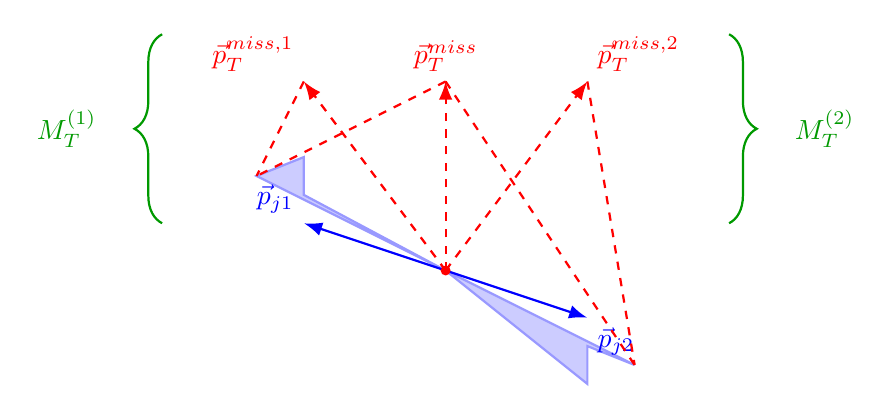
\begin{tikzpicture}[scale=1.2, >=Latex]

% Define coordinates
\coordinate (O) at (0,0); % Vertex
\coordinate (J1) at (-2,1); % Jet 1 tip
\coordinate (J2) at (2,-1); % Jet 2 tip
\coordinate (P1) at (-1.5,2); % Missing momentum 1
\coordinate (P2) at (1.5,2); % Missing momentum 2
\coordinate (P) at (0,2); % Central missing momentum

% Draw jets (cones)
\draw[blue!40, fill=blue!20, thick] (O) -- (J1) -- ++(0.5,0.2) -- ++(0,-0.4) -- cycle;
\draw[blue!40, fill=blue!20, thick] (O) -- (J2) -- ++(-0.5,0.2) -- ++(0,-0.4) -- cycle;

% Draw jet momentum vectors
\draw[blue, thick, ->] (O) -- ++(-1.5,0.5) node[above left] {$\vec{p}_{j1}$};
\draw[blue, thick, ->] (O) -- ++(1.5,-0.5) node[below right] {$\vec{p}_{j2}$};

% Draw missing momentum vectors
\draw[red, thick, dashed, ->] (O) -- (P1) node[above left] {$\vec{p}_{\text{T}}^{\text{miss,1}}$};
\draw[red, thick, dashed, ->] (O) -- (P) node[above] {$\vec{p}_{\text{T}}^{\text{miss}}$};
\draw[red, thick, dashed, ->] (O) -- (P2) node[above right] {$\vec{p}_{\text{T}}^{\text{miss,2}}$};

% Draw dashed lines connecting missing momentum to jet tips (for triangle completion)
\draw[red, thick, dashed] (P1) -- (J1);
\draw[red, thick, dashed] (P) -- (J1);
\draw[red, thick, dashed] (P2) -- (J2);
\draw[red, thick, dashed] (P) -- (J2);

% Draw grouping braces
\draw[green!60!black, thick, decorate, decoration={brace, amplitude=10pt, mirror}] 
  (-3,2.5) -- (-3,0.5) node[midway, left=10pt, xshift=-10pt] {$M_T^{(1)}$};
\draw[green!60!black, thick, decorate, decoration={brace, amplitude=10pt}] 
  (3,2.5) -- (3,0.5) node[midway, right=10pt, xshift=10pt] {$M_T^{(2)}$};

% Add small dots at vertex for clarity
\fill[red] (O) circle (1.5pt);

\end{tikzpicture}
\end{document}